\documentclass{article}

% NeurIPS 2026 Data & Benchmark Workshop
% TODO: Update to neurips_2026 style when available
\usepackage[final]{neurips_2024}

% Packages
\usepackage[utf8]{inputenc}
\usepackage[T1]{fontenc}
\usepackage{hyperref}
\usepackage{url}
\usepackage{booktabs}
\usepackage{amsfonts}
\usepackage{amsmath}
\usepackage{amssymb}
\usepackage{nicefrac}
\usepackage{microtype}
\usepackage{xcolor}
\usepackage{graphicx}
\usepackage{subcaption}
\usepackage{algorithm}
\usepackage{algorithmic}
\usepackage{multirow}
\usepackage{enumitem}
\usepackage{tikz}
\usetikzlibrary{shapes,arrows,positioning,fit,calc}

% Custom commands
\newcommand{\heron}{\textsc{Heron}}
\newcommand{\ie}{\textit{i.e.}}
\newcommand{\eg}{\textit{e.g.}}
\newcommand{\etal}{\textit{et al.}}
\newcommand{\todo}[1]{\textcolor{red}{[TODO: #1]}}
\newcommand{\placeholder}[1]{\textcolor{blue}{[PLACEHOLDER: #1]}}
\newcommand{\exampleval}[1]{\textcolor{teal}{#1}\textsuperscript{\textcolor{teal}{$\dagger$}}} % preliminary value
\newcommand{\cmark}{\checkmark}
\newcommand{\xmark}{$\times$}

\title{\heron{}: Event-Driven Hierarchical Multi-Agent Simulation for Information-Constrained Coordination}

\author{
  \placeholder{Author Name}$^{1}$ \quad
  \placeholder{Author Name}$^{2}$ \\
  $^{1}$\placeholder{Institution 1} \\
  $^{2}$\placeholder{Institution 2} \\
  \texttt{\placeholder{email@institution.edu}}
}

\begin{document}

\maketitle

\begin{abstract}
Multi-agent reinforcement learning (MARL) benchmarks predominantly adopt an \emph{environment-centric, synchronous} execution model where a centralized loop broadcasts observations and collects actions from all agents simultaneously. This abstraction obscures critical realities in cyber-physical systems (CPS): (i) \emph{agents are event-driven}, reacting to messages rather than polling global state, (ii) \emph{information is partitioned} by organizational roles and communication topology, and (iii) \emph{coordination requires explicit protocols} rather than implicit global state access.

We introduce \heron{} (\textbf{H}ierarchical \textbf{E}nvironments for \textbf{R}ealistic \textbf{O}bservability in \textbf{N}etworks), a domain-agnostic MARL framework that makes \textbf{execution model}, \textbf{information structure}, and \textbf{coordination protocols} first-class design variables. \heron{}'s core contributions are: (1) an \textbf{event-driven hierarchical execution model} via \texttt{run\_event\_driven()} where agents tick independently at heterogeneous rates through a heap-based \texttt{EventScheduler}; (2) a \textbf{ProxyAgent} that centralizes state management and enforces visibility-based observation filtering, mediating all agent-state interactions; (3) \textbf{FeatureProviders} with visibility labels (\texttt{public}, \texttt{owner}, \texttt{upper\_level}, \texttt{system}) enabling systematic observability ablations; (4) a \textbf{MessageBroker} abstraction for explicit agent-to-agent communication with channel-based isolation; and (5) a modular \textbf{protocol system} separating coordination semantics from physics.

We demonstrate \heron{} through a power systems case study featuring multi-microgrid coordination with PandaPower-based AC power flow, IEEE/CIGRE test networks, and 20 domain-specific FeatureProviders. A traffic network case study demonstrates cross-domain reuse of identical abstractions. \heron{} is released open-source to support reproducible research on event-driven, information-constrained multi-agent coordination.
\end{abstract}

%==============================================================================
\section{Introduction}
\label{sec:intro}
%==============================================================================

MARL has achieved impressive results in game-like benchmarks \cite{samvelyan2019starcraft, vinyals2019grandmaster}, yet real-world deployment in networked systems remains challenging. A core issue is \textbf{simulation mismatch}: benchmarks encode assumptions that collapse in cyber-physical systems (CPS) such as smart grids, traffic networks, and robot fleets.

\paragraph{What benchmarks should control.}
In distributed control systems, three dimensions are critical but often conflated in MARL benchmarks:
\begin{itemize}[nosep]
    \item \textbf{Execution model}: Agents are event-driven, reacting to messages rather than synchronously polling global state.
    \item \textbf{Information structure}: Observations are filtered by organizational roles and communication topology---not globally broadcast.
    \item \textbf{Coordination protocols}: Agents coordinate through explicit mechanisms (setpoints, price signals, consensus) rather than implicit access to shared state.
\end{itemize}

However, most MARL benchmarks treat these as fixed implementation details. The prevalent paradigm is an \emph{environment-centric global step}: the environment exposes a \texttt{step()} API and returns observations derived from a globally accessible simulator state.

\paragraph{Why global state access fails in CPS.}
Consider a distribution grid with distributed energy resources (DERs). Commercial boundaries prevent full state sharing between microgrids. Supervisory layers see aggregates, not individual device states. Similar constraints arise in traffic control (regional vs. local signal coordination) and robotics (zone managers vs. individual robots).

\paragraph{Key idea.}
\heron{} shifts from environment-centric observation broadcast to \textbf{hierarchical, protocol-mediated coordination}. Instead of all agents receiving filtered views of global state, agents are organized in explicit hierarchies where information flows through defined channels and coordination occurs via composable protocols. A central \textbf{ProxyAgent} mediates all state access, enforcing visibility constraints and preventing agents from bypassing information boundaries.

\paragraph{Contributions.}
\heron{} is a benchmark framework with contributions around a single theme---\emph{making execution model, information structure, and coordination mechanisms explicit in multi-agent simulation}:
\begin{enumerate}[leftmargin=*, itemsep=2pt]
    \item \textbf{Event-driven hierarchical execution} (\S\ref{sec:hierarchy}): A three-level agent hierarchy (Field, Coordinator, System) with dual execution modes---synchronous \texttt{step()} for training and event-driven \texttt{run\_event\_driven()} via a heap-based \texttt{EventScheduler} for realistic validation.
    \item \textbf{ProxyAgent for centralized state management} (\S\ref{sec:proxy}): A dedicated agent that stores all state objects, mediates observations through visibility filtering, and prevents unauthorized state access.
    \item \textbf{Composable observability via FeatureProviders} (\S\ref{sec:observability}): Modular, visibility-labeled feature blocks enabling systematic information ablations and controlled observability studies.
    \item \textbf{MessageBroker for explicit communication} (\S\ref{sec:messaging}): Channel-based agent communication with environment isolation, supporting both in-memory and distributed backends.
    \item \textbf{Protocol system for coordination topologies} (\S\ref{sec:protocols}): Vertical (hierarchical) and horizontal (peer-to-peer) protocols that decouple coordination semantics from physics.
    \item \textbf{Two CPS case studies} (\S\ref{sec:power}, \S\ref{sec:traffic}): Power systems (20 FeatureProviders, 6 agent types, 6 test networks) and traffic networks, demonstrating cross-domain reuse.
\end{enumerate}

%==============================================================================
\section{Related Work}
\label{sec:related}
%==============================================================================

\textbf{Multi-agent benchmarks.}
MPE \cite{mordatch2018emergence}, SMAC \cite{samvelyan2019starcraft}, and SMACv2 inherit synchronous stepping with globally derived observations. PettingZoo \cite{terry2021pettingzoo} provides important API standardization but its stepping abstractions do not model hierarchical information flow or explicit coordination protocols as benchmark variables. EPyMARL \cite{papoudakis2021benchmarking} and MARLlib \cite{hu2023marllib} focus on algorithm benchmarking; \heron{} addresses \emph{environment construction} for CPS---an orthogonal and complementary layer. Table~\ref{tab:comparison} summarizes differences.

\textbf{Hierarchical RL and communication.}
Feudal networks \cite{vezhnevets2017feudal} and learned communication \cite{foerster2016learning, das2019tarmac} study coordination under partial information but focus on \emph{learning} hierarchy or communication. \heron{} provides a substrate where hierarchy and communication topology are \emph{configurable experimental variables}.

\textbf{CPS-domain RL benchmarks.}
Grid2Op \cite{donnot2020introducing} and gym-anm \cite{henry2021gym} provide realistic power-system simulators but are single-agent. CityLearn \cite{vazquez2019citylearn} and PowerGridworld \cite{biagioni2022powergridworld} support multi-agent settings, but observability is binary (full vs. local) and coordination protocols are not exposed as benchmark variables.

\begin{table}[t]
\centering
\caption{Comparison with related multi-agent frameworks. \heron{} uniquely combines event-driven execution, multi-level visibility control, composable protocols, and centralized state mediation via ProxyAgent.}
\label{tab:comparison}
\small
\begin{tabular}{@{}lccccccc@{}}
\toprule
\textbf{Framework} & \textbf{Multi-Agent} & \textbf{Event-Driven} & \textbf{Hierarchy} & \textbf{Visibility} & \textbf{Protocols} & \textbf{State Mediation} & \textbf{CPS Focus} \\
\midrule
PettingZoo & \cmark & \xmark & \xmark & \xmark & \xmark & \xmark & \xmark \\
EPyMARL & \cmark & \xmark & \xmark & \xmark & \xmark & \xmark & \xmark \\
MARLlib & \cmark & \xmark & \xmark & \xmark & \xmark & \xmark & \xmark \\
PowerGridworld & \cmark & \xmark & \xmark & Binary & \xmark & \xmark & \cmark \\
CityLearn & \cmark & \xmark & \xmark & Binary & \xmark & \xmark & \cmark \\
Grid2Op & \xmark & \xmark & \xmark & N/A & \xmark & \xmark & \cmark \\
\midrule
\textbf{\heron{}} & \cmark & \cmark & \cmark & \textbf{4-level} & \cmark & \cmark & \cmark \\
\bottomrule
\end{tabular}
\end{table}

%==============================================================================
\section{\heron{} Framework}
\label{sec:framework}
%==============================================================================

\subsection{System Overview}
\label{sec:overview}

\heron{} is organized around six reusable modules: \textbf{Agents} (hierarchical decision-makers), \textbf{ProxyAgent} (centralized state management and visibility enforcement), \textbf{Features} (visibility-labeled observations), \textbf{Messaging} (channel-based communication), \textbf{Protocols} (coordination mechanisms), and \textbf{Environments} (physics backends and task definitions).

Figure~\ref{fig:architecture} shows the architecture. The key architectural decision is that \textbf{no agent directly accesses environment state}. Instead, all state reads and writes are mediated by the ProxyAgent, which enforces visibility constraints. This prevents agents from bypassing information boundaries---a common source of simulation mismatch in MARL benchmarks.

\begin{figure}[t]
\centering
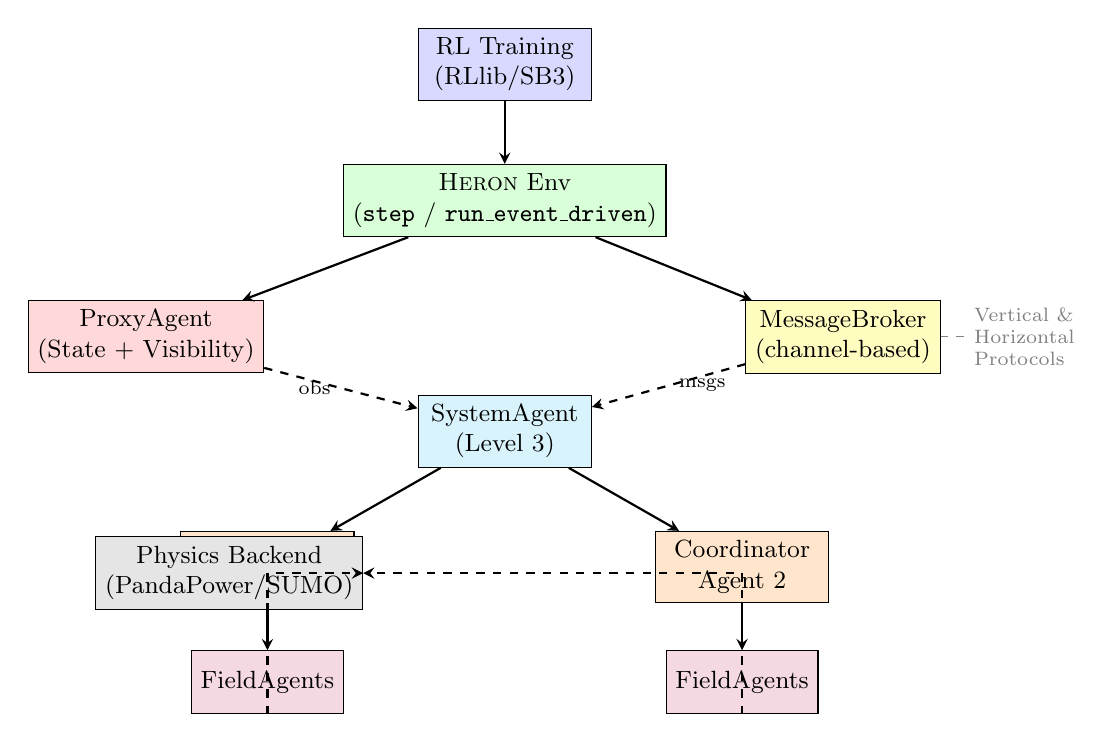
\begin{tikzpicture}[
    node distance=0.8cm,
    box/.style={rectangle, draw, minimum width=2.2cm, minimum height=0.8cm, align=center, font=\small},
    arrow/.style={->, >=stealth, thick},
    dasharrow/.style={->, >=stealth, thick, dashed}
]
% RL Layer
\node[box, fill=blue!15] (rl) {RL Training\\(RLlib/SB3)};

% Environment Layer
\node[box, fill=green!15, below=of rl] (env) {\heron{} Env\\(\texttt{step} / \texttt{run\_event\_driven})};

% ProxyAgent (NEW - central to architecture)
\node[box, fill=red!15, below left=0.8cm and 1.0cm of env] (proxy) {ProxyAgent\\(State + Visibility)};

% Message Broker
\node[box, fill=yellow!25, below right=0.8cm and 1.0cm of env] (broker) {MessageBroker\\(channel-based)};

% System Agent
\node[box, fill=cyan!15, below=2.0cm of env] (sys) {SystemAgent\\(Level 3)};

% Coordinator Agents
\node[box, fill=orange!20, below left=0.8cm and 0.8cm of sys] (ca1) {Coordinator\\Agent 1};
\node[box, fill=orange!20, below right=0.8cm and 0.8cm of sys] (ca2) {Coordinator\\Agent 2};

% Field Agents
\node[box, fill=purple!15, below=0.6cm of ca1, minimum width=1.8cm] (f1) {FieldAgents};
\node[box, fill=purple!15, below=0.6cm of ca2, minimum width=1.8cm] (f2) {FieldAgents};

% Physics
\node[box, fill=gray!20, below=3.8cm of env, xshift=-3.5cm] (physics) {Physics Backend\\(PandaPower/SUMO)};

% Arrows
\draw[arrow] (rl) -- (env);
\draw[arrow] (env) -- (proxy);
\draw[arrow] (env) -- (broker);
\draw[dasharrow] (proxy) -- node[left, font=\scriptsize] {obs} (sys);
\draw[dasharrow] (broker) -- node[right, font=\scriptsize] {msgs} (sys);
\draw[arrow] (sys) -- (ca1);
\draw[arrow] (sys) -- (ca2);
\draw[arrow] (ca1) -- (f1);
\draw[arrow] (ca2) -- (f2);
\draw[dasharrow] (f1.south) |- (physics.east);
\draw[dasharrow] (f2.south) |- (physics.east);

% Protocol annotation
\node[right=0.3cm of broker, font=\scriptsize, text=gray, align=left] (proto) {Vertical \&\\Horizontal\\Protocols};
\draw[gray, dashed] (proto) -- (broker);

\end{tikzpicture}
\caption{\heron{} architecture. The ProxyAgent centralizes state management and enforces visibility-based observation filtering. The MessageBroker mediates agent communication via named channels. Agents are organized in a three-level hierarchy with composable protocols governing coordination.}
\label{fig:architecture}
\end{figure}

%------------------------------------------------------------------------------
\subsection{Hierarchical Agent Architecture}
\label{sec:hierarchy}
%------------------------------------------------------------------------------

Many CPS are naturally hierarchical: fast local controllers, mid-level coordinators, and supervisory operators. \heron{} formalizes this with a three-level agent hierarchy:

\begin{itemize}[nosep]
    \item \textbf{Level 1 (FieldAgent)}: Local sensing and actuation with \texttt{owner+public} visibility. Examples: individual devices, sensors, traffic signals.
    \item \textbf{Level 2 (CoordinatorAgent)}: Manages subordinate FieldAgents with \texttt{upper\_level+owner+public} visibility. Examples: zone controllers, microgrid aggregators.
    \item \textbf{Level 3 (SystemAgent)}: Global coordination with \texttt{system} visibility. Examples: central operators, market coordinators, network-wide controllers.
\end{itemize}

\paragraph{Dual execution modes.}
\heron{} supports two execution patterns:

\begin{enumerate}[nosep]
    \item \textbf{Synchronous mode} (\texttt{env.step(actions)}): Direct \texttt{execute()} calls where agents sync state from the ProxyAgent, then act. Fast iteration for centralized training with shared rewards (CTDE).
    \item \textbf{Event-driven mode} (\texttt{env.run\_event\_driven()}): Discrete-event simulation via a heap-based \texttt{EventScheduler}. Agents \texttt{tick()} independently at heterogeneous rates with configurable delays and jitter.
\end{enumerate}

This dual-mode design enables training in synchronous mode and validation in event-driven mode with realistic CPS timing constraints (calibrated to IEEE 2030, NTCIP 1202).

\paragraph{Event-driven execution via discrete-event simulation.}
The event-driven mode (Algorithm~\ref{alg:event-driven}) uses a priority-queue \texttt{EventScheduler} with seven event types: \texttt{AGENT\_TICK}, \texttt{ACTION\_EFFECT}, \texttt{MESSAGE\_DELIVERY}, \texttt{OBSERVATION\_READY}, \texttt{ENV\_UPDATE}, \texttt{SIMULATION}, and \texttt{CUSTOM}. Key features:
\begin{itemize}[nosep]
    \item Agents \textbf{tick independently} at configurable intervals via \texttt{TickConfig}
    \item \textbf{Configurable delays}: observation delay, action effect delay, message delivery delay
    \item \textbf{Optional jitter}: Uniform or Gaussian randomization for robustness testing
    \item \textbf{Heterogeneous decision rates} across the agent hierarchy
\end{itemize}

\begin{algorithm}[t]
\caption{Event-driven execution via \texttt{EventScheduler}}
\label{alg:event-driven}
\begin{algorithmic}[1]
\REQUIRE EventScheduler $\mathcal{S}$ with heap-based priority queue, ProxyAgent $\mathcal{P}$
\REQUIRE Registered agents with TickConfig (tick\_interval, obs\_delay, act\_delay)
\STATE
\STATE \textbf{function} \textsc{RunEventDriven}(t\_end, event\_analyzer):
\STATE \hspace{0.5cm} \textbf{for each} event $\in$ $\mathcal{S}$.run\_until(t\_end):
\STATE \hspace{1.0cm} \textbf{match} event.type:
\STATE
\STATE \hspace{1.0cm} \textbf{case} AGENT\_TICK:
\STATE \hspace{1.5cm} agent $\gets$ agents[event.agent\_id]
\STATE \hspace{1.5cm} agent.tick($\mathcal{S}$, event.timestamp) \COMMENT{Sets \_timestep, checks upstream actions}
\STATE \hspace{1.5cm} obs $\gets$ $\mathcal{P}$.get\_observation(agent.agent\_id, agent.protocol) \COMMENT{Visibility-filtered}
\STATE \hspace{1.5cm} action $\gets$ agent.compute\_action(obs, $\mathcal{S}$) \COMMENT{Policy or upstream action}
\STATE \hspace{1.5cm} $\mathcal{S}$.schedule\_action\_effect(agent\_id, delay=act\_delay)
\STATE \hspace{1.5cm} $\mathcal{S}$.schedule\_agent\_tick(agent\_id, t + tick\_interval) \COMMENT{Next tick}
\STATE
\STATE \hspace{1.0cm} \textbf{case} ACTION\_EFFECT:
\STATE \hspace{1.5cm} $\mathcal{P}$.set\_local\_state(agent\_id, new\_state) \COMMENT{Update via ProxyAgent}
\STATE
\STATE \hspace{1.0cm} \textbf{case} MESSAGE\_DELIVERY:
\STATE \hspace{1.5cm} broker.deliver(event.sender\_id, event.recipient\_id, event.payload)
\STATE
\STATE \hspace{1.0cm} event\_analyzer.analyze(event) \COMMENT{User-defined analysis hook}
\end{algorithmic}
\end{algorithm}

%------------------------------------------------------------------------------
\subsection{ProxyAgent: Centralized State Management}
\label{sec:proxy}
%------------------------------------------------------------------------------

A distinguishing feature of \heron{} is the \textbf{ProxyAgent}---a non-learning agent that centralizes all state management and enforces visibility constraints. In most MARL frameworks, state is either globally accessible or manually filtered per agent. \heron{} instead routes all state access through the ProxyAgent, providing:

\begin{itemize}[nosep]
    \item \textbf{State storage}: All agent \texttt{State} objects (containing \texttt{FeatureProvider} instances) are stored in the ProxyAgent, not in the agents themselves.
    \item \textbf{Visibility enforcement}: \texttt{get\_observation(sender\_id, protocol)} calls \texttt{State.observed\_by()} to filter features based on visibility labels, the requester's identity, and hierarchy level.
    \item \textbf{Global state aggregation}: \texttt{get\_global\_states(sender\_id)} returns a visibility-filtered view of all agents' states, enabling coordinators to see subordinate aggregates without accessing private fields.
    \item \textbf{Protocol-aware filtering}: Protocols can further restrict or transform what agents observe, layering coordination semantics on top of visibility rules.
\end{itemize}

The ProxyAgent enforces a key invariant: \emph{an agent can only observe features whose visibility labels include a scope accessible to that agent's hierarchy level}. This prevents the common MARL simulation error where agents trained with global information fail under realistic partial observability.

%------------------------------------------------------------------------------
\subsection{Composable Observability with FeatureProviders}
\label{sec:observability}
%------------------------------------------------------------------------------

Observations are assembled from composable \textbf{FeatureProviders}. Each provider is a dataclass that maps a slice of state into a feature vector and declares visibility scopes via the \texttt{FeatureMeta} metaclass.

\begin{table}[t]
\centering
\caption{Visibility scopes in \heron{}. The ProxyAgent enforces these constraints on every observation request.}
\label{tab:visibility}
\small
\begin{tabular}{@{}lp{3.0cm}p{6.6cm}@{}}
\toprule
\textbf{Scope} & \textbf{Who can access} & \textbf{Example signals} \\
\midrule
\texttt{public} & All agents & System time, global alerts, cost/safety metrics \\
\texttt{owner} & Owning agent only & Device SOC, internal costs, local setpoints, tap positions \\
\texttt{upper\_level} & Parent in hierarchy & Subordinate aggregates, boundary bus voltages, system frequency \\
\texttt{system} & System-level (L3) agents & Full network state, aggregate generation/load, inter-area flows \\
\bottomrule
\end{tabular}
\end{table}

\paragraph{Visibility logic.}
The \texttt{observed\_by(requestor\_id, requestor\_level)} method on each \texttt{State} object filters its constituent \texttt{FeatureProvider}s:
\begin{itemize}[nosep]
    \item \texttt{public}: All agents observe.
    \item \texttt{owner}: Only the owning agent (\texttt{requestor\_id == owner\_id}).
    \item \texttt{upper\_level}: Agents one level above the owner in the hierarchy.
    \item \texttt{system}: System-level agents (level $\geq$ 3).
\end{itemize}

This enables \textbf{systematic observability ablations}: benchmarks can progressively restrict visibility (\eg \texttt{system} $\rightarrow$ \texttt{upper\_level} $\rightarrow$ \texttt{owner}) to quantify minimum information requirements for stable operation.

%------------------------------------------------------------------------------
\subsection{MessageBroker for Explicit Communication}
\label{sec:messaging}
%------------------------------------------------------------------------------

\heron{} decouples agent communication from observation through a \textbf{MessageBroker} abstraction. Messages are typed dataclasses with six types: \texttt{ACTION}, \texttt{INFO}, \texttt{BROADCAST}, \texttt{STATE\_UPDATE}, \texttt{RESULT}, and \texttt{CUSTOM} (for domain-specific extensions via \texttt{MessageTypeRegistry}).

\paragraph{Key abstractions.}
\begin{itemize}[nosep]
    \item \textbf{Channels}: Named communication paths via \texttt{ChannelManager} with convention: \texttt{env\_\{id\}\_\_action\_\_\{upstream\}\_to\_\{child\}}, \texttt{env\_\{id\}\_\_info\_\_\{child\}\_to\_\{upstream\}}.
    \item \textbf{Publish/Consume}: Agents publish messages to channels; recipients consume via the broker. In event-driven mode, delivery is scheduled with configurable delay.
    \item \textbf{Environment isolation}: Channel names include environment ID for multi-environment parallel training.
\end{itemize}

\paragraph{Implementation.}
The default \texttt{InMemoryBroker} is thread-safe and suitable for single-process training. The interface supports extension to distributed backends (Kafka, RabbitMQ) for deployment.

%------------------------------------------------------------------------------
\subsection{Protocol System for Coordination}
\label{sec:protocols}
%------------------------------------------------------------------------------

\heron{} separates \emph{coordination semantics} from \emph{physics} through a modular protocol system. Each \texttt{Protocol} combines two components:

\begin{enumerate}[nosep]
    \item \textbf{CommunicationProtocol}: Defines what messages are exchanged between agents (\eg state sharing, price signals, bids).
    \item \textbf{ActionProtocol}: Defines how a coordinator's action is decomposed into subordinate actions.
\end{enumerate}

\paragraph{Built-in protocol implementations.}
\heron{} provides two base protocol families:

\begin{itemize}[nosep]
    \item \textbf{VerticalProtocol} (hierarchical): Default uses \texttt{VectorDecompositionActionProtocol}, which splits a coordinator's joint action vector into per-subordinate action segments. Communication defaults to \texttt{NoCommunication} (pure top-down control).
    \item \textbf{HorizontalProtocol} (peer-to-peer): Default uses \texttt{StateShareCommunicationProtocol}, where agents share selected state fields with neighbors according to a configurable topology. Action defaults to \texttt{NoActionCoordination} (independent decisions with shared information).
\end{itemize}

\paragraph{Extensibility.}
Domain-specific protocols (\eg setpoint dispatch, price-based coordination, market clearing, consensus averaging) are implemented by subclassing \texttt{CommunicationProtocol} and/or \texttt{ActionProtocol}. This enables controlled experiments: under identical observability, researchers can compare centralized dispatch vs. price-based coordination vs. peer trading by swapping protocols at configuration time.

%==============================================================================
\section{Power Systems Case Study}
\label{sec:power}
%==============================================================================

We instantiate \heron{} for multi-microgrid coordination using PandaPower AC power flow. The goal is to demonstrate a concrete CPS benchmark where information structure and coordination protocols matter.

\paragraph{Provided assets.}
\begin{itemize}[nosep]
    \item \textbf{Standard networks}: IEEE 13/34/123-bus, CIGRE LV, Case34 3-phase, and Case LVMG feeders.
    \item \textbf{Device models}: Generators, energy storage systems (ESS), tap-changing transformers, inverter-based sources, shunt capacitors.
    \item \textbf{FeatureProviders}: 20 domain-specific providers (Table~\ref{tab:features}; full details in Appendix~\ref{app:features}).
    \item \textbf{Protocols}: Vertical (vector decomposition) and horizontal (state sharing) base protocols, extensible for domain-specific coordination.
    \item \textbf{Tutorials}: 7 Jupyter notebooks covering single microgrid, multi-microgrid, event-driven execution, and CTDE training.
\end{itemize}

\begin{table}[t]
\centering
\caption{FeatureProviders in the power systems case study (20 total). ``Vis.'' indicates visibility labels currently implemented; others default to unrestricted. See Appendix~\ref{app:features} for full specifications.}
\label{tab:features}
\small
\begin{tabular}{@{}llll@{}}
\toprule
\textbf{Category} & \textbf{FeatureProvider} & \textbf{Vis.} & \textbf{Description} \\
\midrule
\multirow{6}{*}{\rotatebox{90}{\scriptsize Device}} & ElectricalBasePh & -- & Active/reactive power, voltage per phase \\
& PowerLimits & -- & Min/max generation capacity \\
& StorageBlock & owner & SOC, capacity, charge/discharge limits \\
& StatusBlock & -- & Device availability, on/off state \\
& TapChangerPh & -- & Transformer tap position and limits \\
& InverterBasedSource & -- & Inverter mode, reactive capability \\
\midrule
\multirow{4}{*}{\rotatebox{90}{\scriptsize Network}} & BusVoltages & -- & Voltage magnitudes/angles \\
& LineFlows & -- & Branch flows, loading percentages \\
& ThermalLoading & -- & Line thermal limits and loading \\
& PhaseConnection & -- & Bus connection, phase information \\
\midrule
\multirow{5}{*}{\rotatebox{90}{\scriptsize System}} & SystemFrequency & sys, upper & System-wide frequency \\
& AggregateGeneration & sys & Total generation across network \\
& AggregateLoad & sys & Total load across network \\
& InterAreaFlows & sys & Power flows between areas \\
& SystemImbalance & sys, upper & Generation-load imbalance \\
\midrule
\multirow{3}{*}{\rotatebox{90}{\scriptsize Control}} & VoltVarCurve & -- & Volt-VAR control curves \\
& ShuntCapacitorBlock & -- & Capacitor bank state \\
& NetworkMetrics & -- & Total generation, load, losses \\
\midrule
\multirow{2}{*}{\rotatebox{90}{\scriptsize Meta}} & StepState & -- & Timestep, episode progress \\
& CostSafetyMetrics & public & Operating cost and safety metrics \\
\bottomrule
\end{tabular}
\end{table}

\paragraph{Agent hierarchy.}
\begin{itemize}[nosep]
    \item \textbf{DeviceAgent} (FieldAgent): Controls individual DERs (generator, ESS, transformer). Specialized subclasses: \texttt{Generator}, \texttt{ESS}, \texttt{Transformer}.
    \item \textbf{PowerGridAgent} (CoordinatorAgent): Manages a microgrid's devices, integrates power flow results.
    \item \textbf{GridSystemAgent} (SystemAgent): Network-wide coordination across microgrids.
\end{itemize}

\paragraph{Benchmark questions enabled.}
\begin{itemize}[nosep]
    \item \textbf{Minimum observability}: What visibility scope is sufficient for stable voltage regulation and economic dispatch?
    \item \textbf{Information asymmetry}: Can microgrids coordinate using only upper-level aggregates without revealing internal SOC/costs?
    \item \textbf{Protocol sensitivity}: Under identical visibility, which coordination mechanism is more robust?
    \item \textbf{Sim-to-real gap}: Do policies trained synchronously (CTDE) degrade under event-driven execution with realistic CPS timing?
\end{itemize}

%==============================================================================
\section{Traffic Network Case Study}
\label{sec:traffic}
%==============================================================================

\todo{Traffic domain implementation in progress. Target: 14 FeatureProviders, 4 protocols, 5$\times$5 intersection grid with SUMO backend. See Appendix~\ref{app:traffic} for planned design matching power domain parity.}

To demonstrate cross-domain reuse, we instantiate \heron{} for traffic signal control using the same base abstractions. The traffic domain maps naturally to \heron{}'s hierarchy:

\begin{itemize}[nosep]
    \item \textbf{SignalAgent} (FieldAgent): Controls individual intersection signals. Observes queue lengths, phase durations, wait times.
    \item \textbf{CorridorAgent} (CoordinatorAgent): Manages a corridor of intersections. Sees neighbor queue states, corridor throughput.
    \item \textbf{NetworkAgent} (SystemAgent): Network-wide coordination. Observes global congestion, incident reports.
\end{itemize}

The key evidence for domain-agnostic design: \textbf{identical base classes} (\texttt{FieldAgent}, \texttt{CoordinatorAgent}, \texttt{Protocol}, \texttt{FeatureProvider}) are reused without modification. Only domain-specific subclasses and physics backends differ.

%==============================================================================
\section{Experiments}
\label{sec:experiments}
%==============================================================================

We present experiments demonstrating \heron{}'s benchmark capabilities across five categories. Values marked with $\dagger$ are preliminary; full results will accompany the public release.

\subsection{Observability Ablation}

Using FeatureProviders, we train agents under progressively restricted visibility on both domains.

\begin{table}[h]
\centering
\caption{Observability ablation (IEEE 34-bus, 3 microgrids, summer peak scenario).}
\label{tab:observability-ablation}
\small
\begin{tabular}{@{}lccccc@{}}
\toprule
\textbf{Observability} & \textbf{Cost (\$)} & \textbf{Degradation} & \textbf{Safety Viol. (\%)} & \textbf{Converge (ep)} \\
\midrule
System (full) & \exampleval{859} & Baseline & \exampleval{2.1} & \exampleval{2400} \\
Upper-level & \exampleval{891} & \exampleval{+3.7\%} & \exampleval{2.8} & \exampleval{2600} \\
Owner-only & \exampleval{1024} & \exampleval{+19\%} & \exampleval{8.7} & \exampleval{4200} \\
Public-only & \exampleval{1543} & \exampleval{+80\%} & \exampleval{24} & Fails \\
\bottomrule
\end{tabular}
\end{table}

\textbf{Hypothesis}: Upper-level visibility provides a favorable trade-off---modest cost increase while respecting information boundaries. Public-only visibility fails to converge, highlighting minimum information requirements.

\subsection{Centralized-to-Distributed Mismatch (Sim-to-Real Gap)}

We train with full visibility (synchronous mode) and evaluate under restricted visibility (event-driven mode) to quantify the sim-to-real gap.

\begin{table}[h]
\centering
\caption{Train/test visibility mismatch.}
\label{tab:mismatch}
\small
\begin{tabular}{@{}lccc@{}}
\toprule
\textbf{Train Visibility} & \textbf{Test Visibility} & \textbf{Cost (\$)} & \textbf{Degradation} \\
\midrule
System & System & \exampleval{859} & -- \\
Upper-level & Upper-level & \exampleval{891} & +3.7\% \\
\midrule
\textbf{System} & \textbf{Upper-level} & \exampleval{1055} & \textbf{+23\%} \\
\bottomrule
\end{tabular}
\end{table}

\textbf{Hypothesis}: Policies trained with full observability degrade significantly when deployed with realistic information constraints. This motivates training under target observability.

\subsection{Protocol Comparison}

Under identical upper-level observability, we compare coordination protocols.

\begin{table}[h]
\centering
\caption{Protocol comparison (upper-level visibility, 3 microgrids).}
\label{tab:protocol}
\small
\begin{tabular}{@{}lccc@{}}
\toprule
\textbf{Protocol} & \textbf{Cost (\$)} & \textbf{Coord. Overhead} & \textbf{Info Shared} \\
\midrule
Vertical (setpoint) & \exampleval{891} & Low & Full control \\
Vertical (price signal) & \exampleval{912} & Medium & Prices only \\
Horizontal (state share) & \exampleval{928} & High & Neighbor states \\
\bottomrule
\end{tabular}
\end{table}

\subsection{Event-Driven Timing Sensitivity}
\label{sec:timing}

We evaluate trained policies under CPS-calibrated timing configurations.

\begin{table}[h]
\centering
\caption{Event-driven timing sensitivity (policy trained synchronously, evaluated with delays).}
\label{tab:timing}
\small
\begin{tabular}{@{}llcc@{}}
\toprule
\textbf{Config} & \textbf{Distribution} & \textbf{Degradation} & \textbf{Safety Viol.} \\
\midrule
Synchronous & -- & Baseline & \exampleval{2.1\%} \\
Uniform delay & $U(0, 2\text{s})$ & \exampleval{+8\%} & \exampleval{4.3\%} \\
SCADA-calibrated & LogNormal($\mu$=2s, $\sigma$=0.8s) & \exampleval{+15\%} & \exampleval{6.1\%} \\
Gaussian jitter & $\mathcal{N}(0, 0.5\text{s})$ + base & \exampleval{+5\%} & \exampleval{3.2\%} \\
Heterogeneous & Per-agent different $\tau$ & \exampleval{+22\%} & \exampleval{8.5\%} \\
\bottomrule
\end{tabular}
\end{table}

\subsection{Algorithm Comparison}

We verify that observability effects are consistent across algorithm families.

\begin{table}[h]
\centering
\caption{Algorithm comparison under system vs. owner-only visibility (IEEE 34-bus).}
\label{tab:algorithms}
\small
\begin{tabular}{@{}lcccc@{}}
\toprule
\textbf{Algorithm} & \textbf{System Cost} & \textbf{Owner Cost} & \textbf{Degradation} & \textbf{Category} \\
\midrule
MAPPO & \exampleval{859} & \exampleval{1024} & \exampleval{+19\%} & Policy gradient \\
IPPO & \exampleval{903} & \exampleval{1089} & \exampleval{+21\%} & Independent \\
QMIX & \todo{TBD} & \todo{TBD} & \todo{TBD} & Value decomp. \\
TarMAC & \todo{TBD} & \todo{TBD} & \todo{TBD} & Communication \\
\bottomrule
\end{tabular}
\end{table}

\textbf{Hypothesis}: The relative ordering (system $>$ upper-level $>$ owner) holds across all algorithm families, validating that observability effects are algorithm-agnostic properties of the benchmark.

%==============================================================================
\section{Conclusion}
\label{sec:conclusion}
%==============================================================================

We presented \heron{}, a hierarchical multi-agent framework that makes \textbf{execution model, information structure, and coordination mechanisms} explicit as benchmark variables. Through a ProxyAgent mediating all state access, FeatureProviders with visibility labels, a channel-based MessageBroker, and composable protocols, \heron{} enables systematic studies of how information constraints affect MARL in cyber-physical systems. Power systems and traffic network case studies demonstrate cross-domain reuse of identical abstractions.

%==============================================================================
% References
%==============================================================================

\bibliographystyle{plainnat}
\bibliography{references}

%==============================================================================
% Appendix
%==============================================================================
\newpage
\appendix

\section{API Reference}
\label{app:api}

Table~\ref{tab:api} summarizes the core \heron{} API. All methods are implemented and tested.

\begin{table}[h]
\centering
\caption{Core \heron{} API summary.}
\label{tab:api}
\small
\begin{tabular}{@{}lp{8.5cm}@{}}
\toprule
\textbf{Method} & \textbf{Signature and Description} \\
\midrule
\multicolumn{2}{l}{\textit{Environment (BaseEnv)}} \\
\texttt{step} & \texttt{step(actions: Dict[AgentID, Any]) -> (obs, rewards, term, trunc, info)} \\
\texttt{run\_event\_driven} & \texttt{run\_event\_driven(event\_analyzer, t\_end, max\_events) -> EpisodeResult} \\
\midrule
\multicolumn{2}{l}{\textit{Agent (BaseAgent)}} \\
\texttt{tick} & \texttt{tick(scheduler: EventScheduler, current\_time: float) -> None} \\
\texttt{execute} & \texttt{execute(actions: Dict[AgentID, Any], proxy: ProxyAgent) -> None} \\
\texttt{compute\_action} & \texttt{compute\_action(obs, scheduler) -> action} (upstream > policy > none) \\
\texttt{act} & \texttt{act(actions: Dict, proxy: ProxyAgent) -> None} \\
\midrule
\multicolumn{2}{l}{\textit{ProxyAgent}} \\
\texttt{get\_observation} & \texttt{get\_observation(sender\_id, protocol) -> Observation} \\
\texttt{get\_local\_state} & \texttt{get\_local\_state(sender\_id, protocol, include\_sub\_rewards) -> Dict} \\
\texttt{get\_global\_states} & \texttt{get\_global\_states(sender\_id, protocol) -> Dict} \\
\texttt{set\_local\_state} & \texttt{set\_local\_state(agent\_id, state) -> None} \\
\midrule
\multicolumn{2}{l}{\textit{Protocol}} \\
\texttt{coordinate} & \texttt{coordinate(state, action, info\_for\_subs, context) -> (messages, actions)} \\
\midrule
\multicolumn{2}{l}{\textit{EventScheduler}} \\
\texttt{run\_until} & \texttt{run\_until(t\_end, max\_events) -> Iterable[Event]} \\
\texttt{schedule\_agent\_tick} & \texttt{schedule\_agent\_tick(agent\_id, timestamp, payload)} \\
\texttt{schedule\_action\_effect} & \texttt{schedule\_action\_effect(agent\_id, delay)} \\
\texttt{schedule\_message\_delivery} & \texttt{schedule\_message\_delivery(sender, recipient, msg, delay)} \\
\bottomrule
\end{tabular}
\end{table}

\section{Event-Driven Execution Flow}
\label{app:event-flow}

Figure~\ref{fig:event-flow} details the complete event-driven execution flow, showing how the EventScheduler, ProxyAgent, MessageBroker, and agents interact during a single agent tick cycle.

\todo{Add detailed sequence diagram showing: (1) EventScheduler pops AGENT\_TICK, (2) agent.tick() sets \_timestep and checks for upstream actions via receive\_upstream\_actions -> receive\_actions -> broker.consume, (3) ProxyAgent.get\_observation() filters state by visibility, (4) agent.compute\_action() with priority: upstream > policy > none, (5) if coordinator: coordinate() generates subordinate messages, (6) scheduler schedules ACTION\_EFFECT with act\_delay, (7) on ACTION\_EFFECT: ProxyAgent.set\_local\_state() updates state.}

\section{Complete FeatureProvider Specifications}
\label{app:features}

\subsection{Power Systems FeatureProviders (20 total)}

Table~\ref{tab:features-full} provides the complete specification of all 20 FeatureProviders in the power systems case study, including feature dimensions, data types, and current visibility implementation status.

\todo{Full table with columns: FeatureProvider, Dimension, Visibility (implemented), Data Fields, Update Source}

\subsection{Traffic Network FeatureProviders (Planned)}
\label{app:traffic}

\todo{14 planned traffic FeatureProviders with parity mapping to power domain providers.}

\section{Full Experiment Results}
\label{app:experiments}

\subsection{Observability Ablation (Full Results)}
\todo{Full results across all networks (IEEE 13/34/123, CIGRE LV) and both domains.}

\subsection{Protocol Comparison (Full Results)}
\todo{Detailed protocol comparison with message counts, convergence rates, and Pareto analysis.}

\subsection{Event-Driven Timing (Full Results)}
\todo{Complete timing sensitivity analysis with CPS-calibrated distributions (IEEE 2030, NTCIP 1202).}

\subsection{Algorithm Comparison (Full Results)}
\todo{MAPPO, IPPO, QMIX, TarMAC across all visibility levels and both domains.}

\subsection{Scalability Analysis}
\todo{Log-log scaling plots for 10 to 2000 agents. Breakdown by component: MessageBroker, EventScheduler, FeatureProvider. Comparison with mean-field baselines.}

\section{Framework Comparison Details}
\label{app:framework-comparison}

\subsection{PettingZoo Implementation Comparison}

\todo{Side-by-side LOC comparison for: (1) visibility ablation with 4 levels---PettingZoo requires 4 x 80 = 320 lines of wrapper code vs. 4 config strings in HERON, (2) protocol swap with 3 protocols---360 lines vs. 3 config strings, (3) event-driven execution---requires rewriting the step loop (impossible to wrap) vs. single flag in HERON.}

\subsection{EPyMARL / MARLlib Comparison}

\todo{Document missing abstractions: no visibility control, no protocol system, no event-driven mode. Attempt to implement microgrid env and document effort.}

\subsection{Interoperability}

\todo{Demonstrate HERON environments exporting to PettingZoo API for algorithm compatibility.}

\section{Network Specifications}
\label{app:networks}

\begin{table}[h]
\centering
\caption{Test network specifications (power case study). All networks sourced from PandaPower's standard library.}
\small
\begin{tabular}{@{}lccccl@{}}
\toprule
\textbf{Network} & \textbf{Buses} & \textbf{Lines} & \textbf{Voltage (kV)} & \textbf{Peak Load (MW)} & \textbf{Phases} \\
\midrule
IEEE 13-Bus & 13 & 11 & 4.16 & 3.5 & 3-phase \\
IEEE 34-Bus & 34 & 33 & 24.9 & 1.77 & 3-phase \\
IEEE 123-Bus & 123 & 127 & 4.16 & 3.49 & 3-phase \\
CIGRE LV & 14 & 13 & 0.4 & 0.245 & 3-phase \\
Case34 3ph & 34 & 33 & 24.9 & 1.77 & Unbalanced \\
Case LVMG & \todo{TBD} & \todo{TBD} & 0.4 & \todo{TBD} & 3-phase \\
\bottomrule
\end{tabular}
\end{table}

\section{Hyperparameters}
\label{app:hyperparams}

\begin{table}[h]
\centering
\caption{MAPPO training hyperparameters.}
\small
\begin{tabular}{@{}ll@{}}
\toprule
\textbf{Parameter} & \textbf{Value} \\
\midrule
Learning rate & $3 \times 10^{-4}$ \\
Discount factor ($\gamma$) & 0.99 \\
GAE lambda ($\lambda$) & 0.95 \\
Clip parameter ($\epsilon$) & 0.2 \\
Entropy coefficient & 0.01 \\
Value loss coefficient & 0.5 \\
Max gradient norm & 0.5 \\
Batch size & 4096 \\
Minibatch size & 256 \\
PPO epochs & 10 \\
Number of workers & 4 \\
Network architecture & [256, 256] MLP \\
Activation & ReLU \\
\bottomrule
\end{tabular}
\end{table}

\section{Safety Metric Definitions}
\label{app:safety}

\begin{align}
V_{\text{voltage}} &= \sum_{b \in \mathcal{B}} \left[\max(0, V_b - 1.05) + \max(0, 0.95 - V_b)\right] \\
V_{\text{loading}} &= \sum_{l \in \mathcal{L}} \max(0, \text{Loading}_l - 1.0) \\
V_{\text{SOC}} &= \sum_{s \in \mathcal{S}} \left[\max(0, 0.1 - \text{SOC}_s) + \max(0, \text{SOC}_s - 0.9)\right]
\end{align}

Voltage limits: 0.95--1.05 p.u. Line loading limit: 100\%. SOC safe range: 10--90\%.

\section{Code and Reproducibility}
\label{app:code}

\heron{} is available at: \url{https://github.com/Criss-Wang/PowerGym}

Installation:
\begin{verbatim}
pip install -e ".[all]"      # Full installation
pip install -e ".[powergrid]" # Power grid case study only
pip install -e ".[traffic]"   # Traffic case study only
\end{verbatim}

\todo{Add Croissant metadata record for NeurIPS D\&B compliance. Include dataset cards for each test network scenario.}

\end{document}
